\documentclass{vivid_layout}

% \makeprint is for printing and trimming on paper, w/crop marks.
% \makeprint

%% Required to build cover page
\title{\fontsize{32pt}{15pt}\selectfont Best Practices For Architecting}{\fontsize{30.2pt}{15pt}\selectfont Highly Monitorable Applications}
\date{\color{white} \today{} \textbullet{} Revision 1}
\cover{architecture-monitoring/cover}

%% Required to build "Meet the Author"
\author{Baron Schwartz}{img/baron}

%% Required image for "About VividCortex"
\aboutvc{img/presenter}
\nopagebreak
%% Required resource info
\resourceleft%
	{Practical Scalability Analysis with the Universal Scalability Law}
	{The Universal Scalability Law models how systems perform as they grow. This
	52-page book shows how to use it for practical
	purposes such as capacity planning.}
	{img/scalability}
	{https://www.vividcortex.com/resources/universal-scalability-law/}
\resourceright%
	{Case Study: Tradesy}
	{After deploying VividCortex, Tradesy reported
	``We were able to bring maximum CPU utilization spikes down from 80\% to
	10\%. VividCortex is incredibly straightforward---it's the best MySQL tool I’ve ever used to monitor and analyze databases.''}
	{img/tradesy-thumbnail}
	{https://www.vividcortex.com/resources/tradesy/}

\begin{document}
\maketitle		% Build the cover page
\begin{bio}		% Biographical info for "Meet the Author"
Baron is a performance and scalability expert who participates in various
database, opensource, and distributed systems communities. He has helped build
and scale many large, high-traffic services for Fortune 1000 clients. He has
written several books, including O'Reilly's best-selling High Performance MySQL.
Baron has a CS degree from the University of Virginia.
\end{bio}
\tableofcontents	% Build the table of contents

\section{Introduction}

Is your application easy to monitor in production? Many applications are, but
sadly, some applications are designed with observability as an afterthought.
Consequences include problems such as:

\begin{itemize}
\item It's cost-prohibitive to monitor the app.
\item No existing systems can monitor the app, so you are forced to develop
something custom.
\item The app's instrumentation is lacking, incompatible with popular monitoring
systems, or impossible to correlate with other metrics.
\item Adding instrumentation proves impossible, and you have no visibility.
\item People, processes, or systems related to monitoring become a bottleneck for the organization.
\end{itemize}

Monitoring is one of many important factors of running apps at scale, and just
like backups, security, auditability, and the like, it should ideally be
considered in advance. In this way, you can make the tradeoffs consciously instead
of accidentally.

This ebook collects the experience of a variety of experienced architects and
combines it with what customers have taught us about monitoring at
VividCortex. My hope is that you will be able to apply the best practices in
this book to avoid pitfalls later, and create a highly monitorable
architecture for your application, so you can get excellent visibility with
minimal cost and effort. 

My experience skews towards database
monitoring needs. However, database monitoring 
is a proper superset of general system monitoring, so the lessons
contained in this ebook should apply to a variety of monitoring practices.

\newpage

\section{What Should You Monitor?}

One of the first things people ask when setting up and configuring
monitoring systems is ``what should I monitor?'' This is an excellent guiding
question to use for planning a highly monitorable application. I've given
presentations on this topic, explaining my overall framework for understanding
what metrics systems expose, what those metrics mean, and why it's not ideal
to use that as a starting point. To learn more about this, you can
\href{https://www.youtube.com/watch?v=zLjhFrUhqxg}{listen to a recording of my
Velocity talk}. 
Others have referenced and expanded this material too, including for example
\href{https://www.datadoghq.com/blog/monitoring-101-collecting-data/}{Datadog's
Monitoring 101 Series}.

The gist of those materials is this: you should not let the tail wag the dog in
monitoring. Decide what information you need, which falls into categories
such as work, resources, and events. Then plan to collect (or build
in the ability to measure and expose) that information.

In databases, in particular, the most important thing to measure is queries (or
statements, or requests, or similar).  Queries are the database's unit of work.
From a user's perspective, the query needs to complete correctly and quickly,
and little else matters.  If you're not monitoring queries at a highly granular
level, your database is little more than a black box.  From the operator's perspective,
resource usage is also a primary type of monitoring data.

It turns out that query monitoring is hard no matter how you do it, but you can
certainly make it even harder, and in this book I'll
spend some time discussing how to avoid that issue.

Executing a process is one of the OS's main jobs, so it's
again it's important to measure processes and their work and
resources. The OS is also responsible for managing the process's
interface and communication with the outside world, as well as its access to
resources, so those are particularly relevant too. And finally, the interplay
of the processes and all of those resources is where problems often occur.

So far we've considered ``canned'' software---the database and the OS---but what
about \emph{your} software, the code you write and deploy? Yes, that needs to be
monitorable too, and the same principles apply. Your code has work to do, and
you need to measure and record that. It manages resources and has queues and
interactions, and those are where many issues arise, so measure that too.

It's a lot to do, and you can't possibly do or plan for it all in advance.
That's why this book's focus is much more on \emph{guidelines} than on 
lists of metrics or recipes and the like. As we dive deep, you'll see
more examples that can illustrate specific cases and hopefully provide
principles you can apply broadly.

\section{Observability Tradeoffs}

Monitoring, like any other function of an application, is a set of
tradeoffs among many competing priorities in a high-dimensional space. In this
section, I'll discuss some of those tradeoffs in hopes of helping you make
choices that will lead to better outcomes.

Here are a few of the most important tradeoffs I've seen:

\begin{description}

\item[Developer Friendliness vs. Operability] If you build your application to be
developer friendly, but ignore how it runs in production, you'll
likely end up with an app that is harder to deploy, operate, and monitor. These need not
be mutually exclusive goals---but if operability is an afterthought, you might
make many decisions that \emph{do} preclude choices later.

\item[Your Process vs. Their Software] All software, including monitoring
systems, expresses a worldview and workflow. When these don't match your own,
the choice is which gives: do you adopt your systems and practices to fit into
the monitoring software, or do you require it to support your workflow?

\item[Cost vs. Visibility] In many cases, the more observable a system is, the
more expensive it is to monitor. This follows rather directly from the amount of
monitoring data you can collect from the system and the granularity at which you
collect it. Monitoring can be expensive if you collect a lot of data, but it can
pay off. I've heard that Netflix's monitoring systems are a double-digit
percentage of their overall operating budget. Netflix has even been described as
a monitoring company that happens to stream movies. At the same time, Netflix's
revenue per employee is one of the highest among publicly traded companies.
Coincidence? You decide.

As another example, I know of many companies migrating from Oracle to PostgreSQL
for cost reasons. The licensing cost is certainly much lower, but there's 
no comparison between the amount of visibility Oracle provides and what you can
get in PostgreSQL. Is the compromise worth it? That's a decision you have to
make.

\item[Isolated Services vs. Monoliths] Microservices architectures are all the
rage at the moment. We're big fans of some of the principles of microservices at
VividCortex. But we've seen many customers struggle with the
implications of monitoring microservices, especially when taken to extremes.
Many small pieces create many sources of metrics, which means many metrics, which
makes sophisticated monitoring systems a must. Likewise, lots of metrics leads
to high cost, which I addressed in the previous point (cost versus
visibility).

This point also applies to another current hot topic, containerization. If you
ship tons of Docker containers and run lots of them in production, you have that
many more things to monitor. Likewise, whether you isolate every different
workload onto different databases, or you have some databases that handle
multiple workloads---or even whether you want to run a few big powerful database
servers versus lots and lots of small cheap ones.

Cost and scale of metrics is not a small consideration; depending on the monitoring system you want
to use, you might either find that you're forced to move to a more scalable
alternative; invest insane amounts of time, money, and hardware; or spend
through the nose. Monitoring isn't cheap no matter how you slice it, and when
you multiply the number of ``things'' in your architecture by N, you 
are multiplying your monitoring costs too.

Any shared or combined resource might amortize the monitoring cost, but
at the same time, it might reduce visibility. If you don't use containers, and a
server runs many different kinds of services, then which one of them is
responsible for a spike in network traffic or disk IO from that server? It might
be hard to tell. (VividCortex has per-process metrics on CPU, IO, and the like;
but not all monitoring systems are capable of providing this level of
granularity).

\item[Built-In Metrics vs. By Hook Or By Crook] If the software doesn't provide
much visibility into the metrics you want, what lengths are you willing
to go to get it? At VividCortex, for example, we've decided not to compromise on
query-level visibility, which is why we use TCP traffic capture and decoding to
measure every query a database gets over the network---and we don't need the
database's cooperation to do this because the packet capture is an OS facility.
TCP traffic capture is hard, and we don't recommend you build your own.
But you might be able to do things like DTrace probes to capture your systems'
work if they don't expose what you want to measure. It's just a matter of how
important it is to you.

\end{description}

These are not exhaustive, but hopefully, it's a good sample to illustrate some of
the tradeoffs.

In my opinion, perhaps the most important set of tradeoffs is how you instrument
your custom application code. You can see this clearly in a quadrant diagram of two
continuums:
\begin{center}
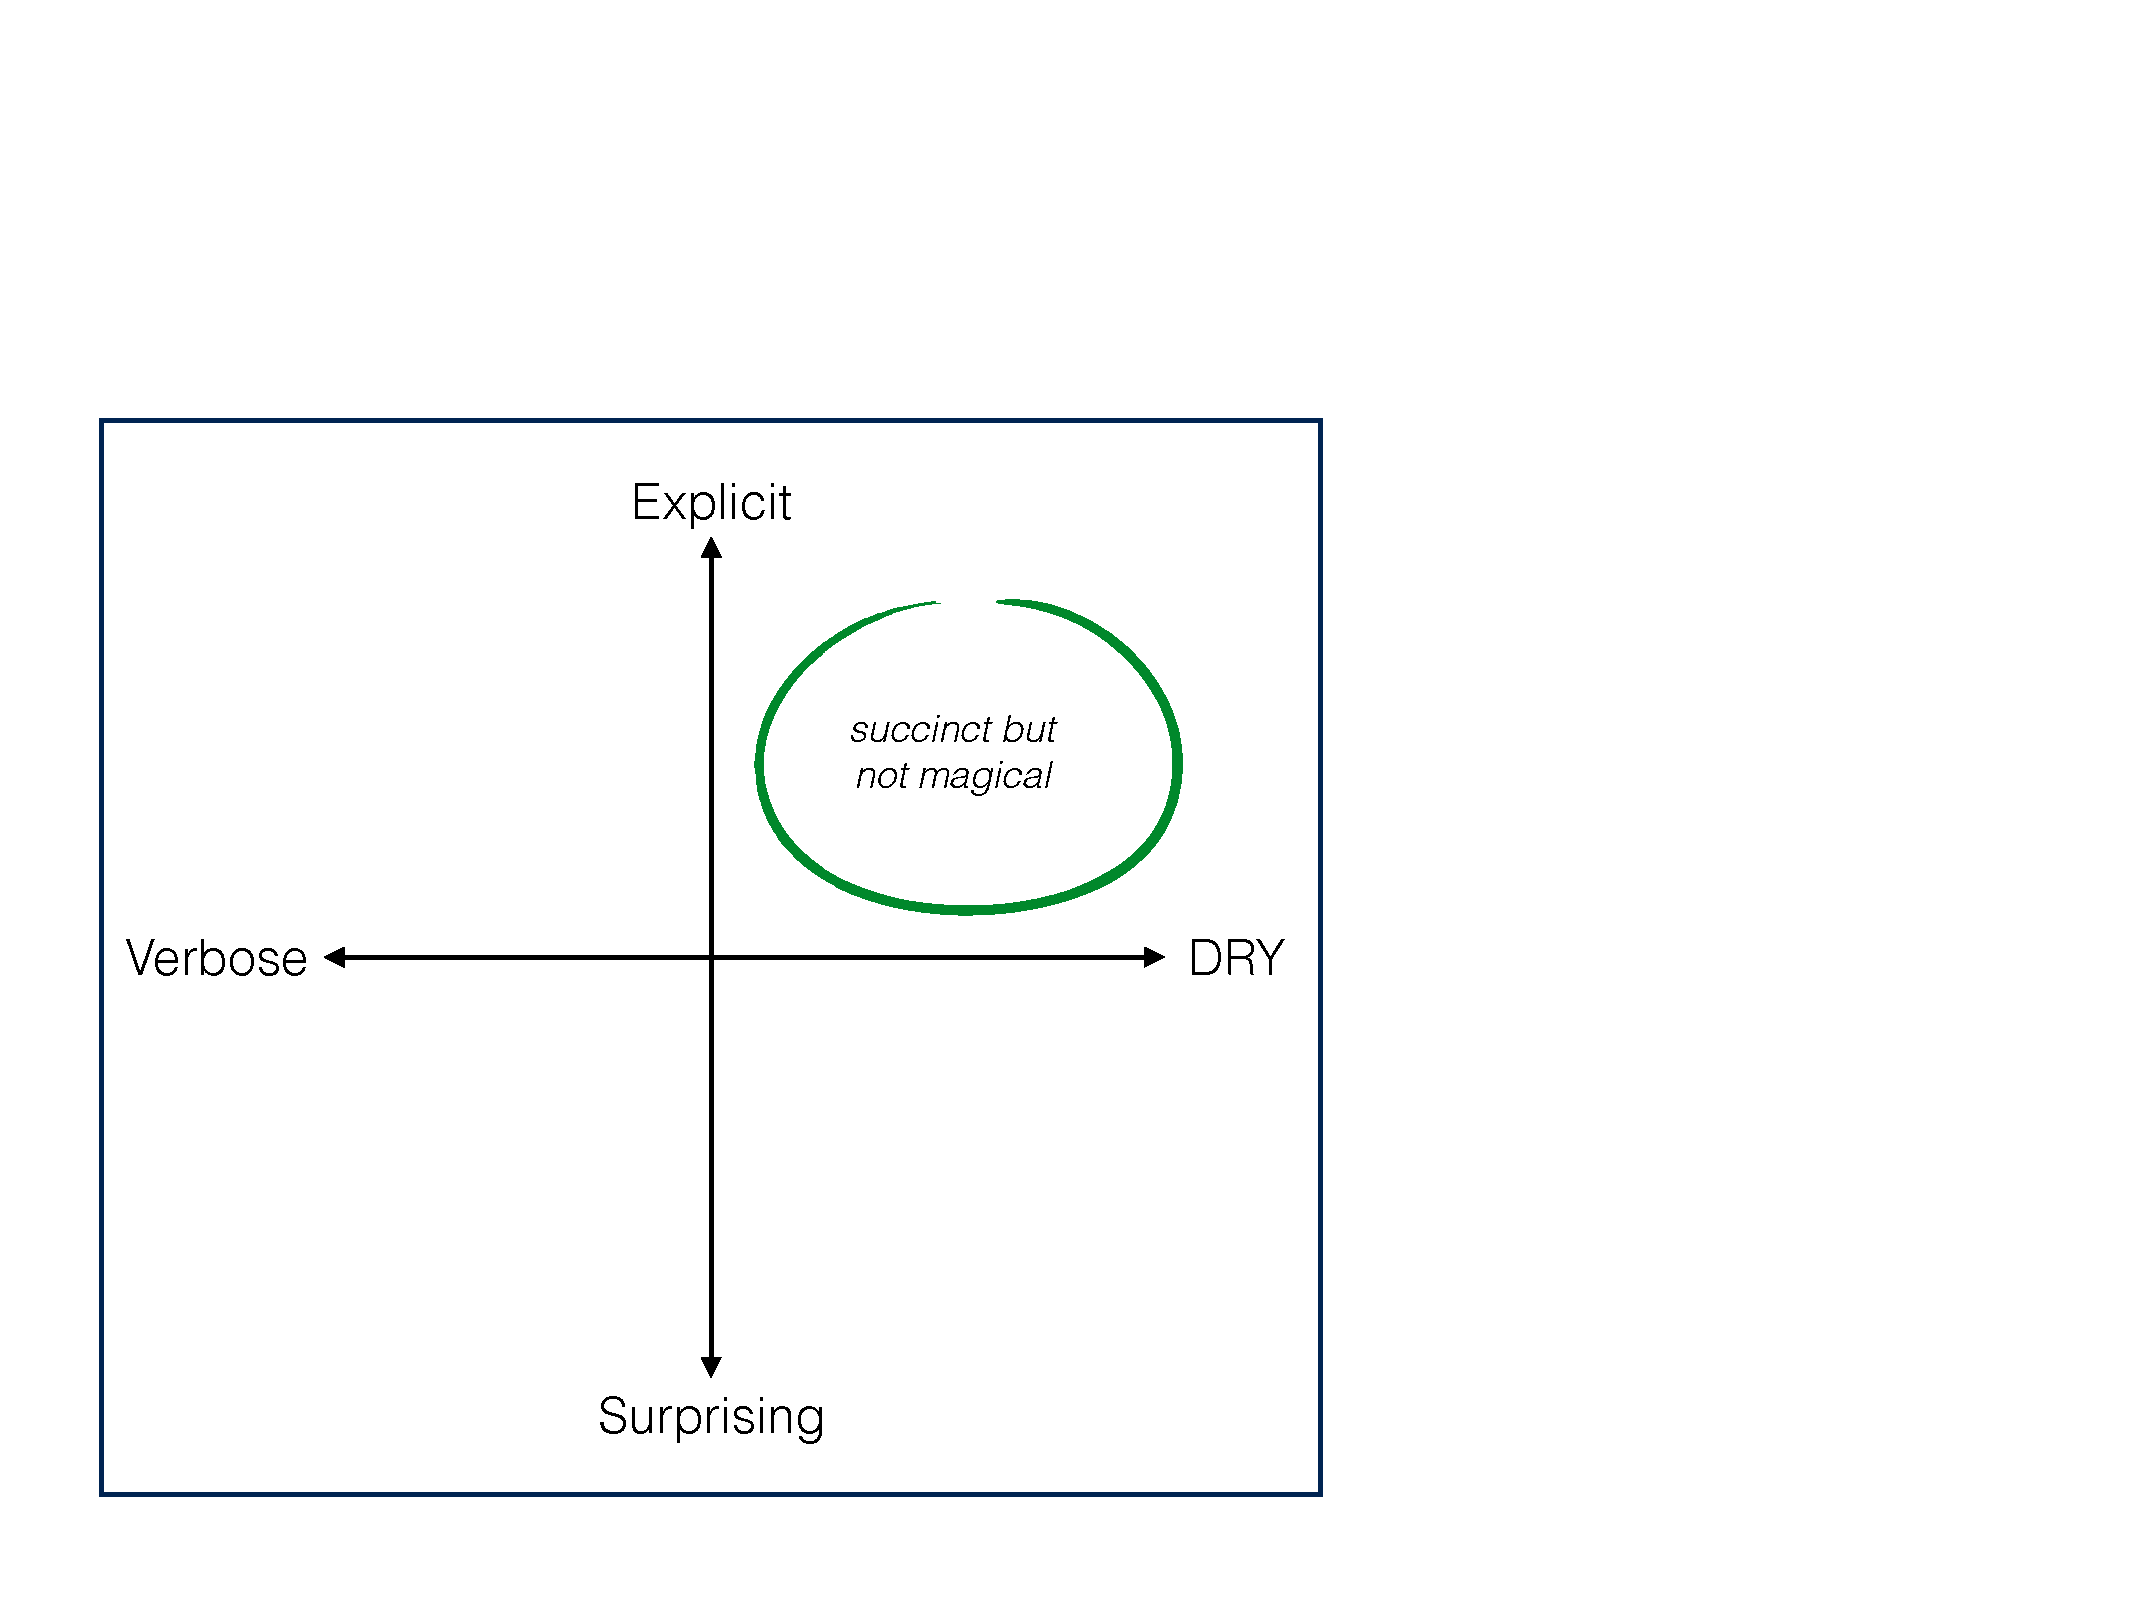
\includegraphics[width=.85\linewidth]{architecture-monitoring/coc}
\end{center}

These are the same two dimensions at play in the principle of
\href{https://en.wikipedia.org/wiki/Convention\_over\_configuration}{convention
over configuration}. The idea is that you'd like code to be consistently and
intuitively instrumented and observable with minimal developer effort, yet have
that instrumentation be flexible if you want or need to change it.
It's a goal that frameworks can help you achieve in some cases.

\section{Service Ownership}

Pick a service in your application. Who's responsible for running it in
production? Is it the same people who wrote it?

One of the core tenets of DevOps, which aligns well with microservices
architectures, is that those who write the code are responsible for making sure
it runs well in production too. This requires that they be
able to monitor it in production.

This book isn't the place to dive deeply into the many valid reasons for this
viewpoint. But I do want to point out one of the main ways in which
silos hurt performance and reliability: the absence or interruption of feedback
loops. If a developer doesn't have to operate their systems in production, they
will not make those systems easy to operate. It's that simple. They won't know
what types of affordances those systems need; they won't know which log messages
are helpful or which are missing; and so on. Operability is a feature, and they
won't know how to make that feature work well.

If you buy into this argument, it's quite clear that every service running in
production needs to be monitored and logged, and the metrics and log events need
to be accessible to people who have better things to do than SSH into
servers. Application and system metrics need to be transparent, discoverable,
and defined with the code so that deploying the code also deploys any necessary
interconnects with monitoring services.

\section{Common Monitoring Pitfalls}

In this section, I'll explore some of the problems I've seen, both in custom
software and in off-the-shelf systems, on monitorability and how it
is designed into or derived from those systems. To begin with, here are some
topics that are mostly related to custom application code, but are also good
advice for anyone building server software for someone else to use:

\begin{description}

\item[Log Levels] There never seem to be enough logging levels to 
capture the desired granularity and relevance of a log message accurately. Is it INFO,
TRACE, or DEBUG? What if it's DEBUG but it's for a condition we should WARN
about? Is there really a linear hierarchy here? And if you're like most people,
you've seen at least once an extension of those types of standard logging levels
on top of a widely available logging system to add \emph{even more} custom
levels. I think there's a good argument that there should be only two
types of log messages: those useful for writing and debugging the code, and
those useful for operating it. Dave Cheney has a
\href{http://dave.cheney.net/2015/11/05/lets-talk-about-logging}{good blog post}
about this.

\item[Mixed Status and Configuration] Many systems don't distinguish between
status variables, which signal the system's state, and configuration variables,
which are inputs to the system's operation. For example, in both MySQL and
Redis, the commands to get system status will return mixtures of configuration
variables and status metrics. Such a metrics ``melting pot'' is a very common problem that usually
requires custom code or exception lists (blacklist/whitelist) to identify which
variables are what.

\item[Breaking Backwards Compatibility] If you change the meaning or dimensions
of a metric, ideally you should leave the old behavior unchanged and introduce a
replacement alongside it. Failure to do this causes a lot of work for other
systems. For example, in MySQL, the SHOW STATUS command was changed to include
connection-specific counters by default, with the old system-wide global
counters accessible via a different query syntax. This change was just a bad decision,
and it caused an enormous amount of grief. Likewise, the meaning of MySQL's
``Questions'' status variable was changed at one point, and the old behavior was
available in a new variable called ``Queries.'' Essentially, they
\href{http://dev.mysql.com/doc/refman/5.0/en/server-status-variables.html#statvar\_Questions}{renamed
a variable and then introduced a new, different variable with the same name as
the old one}. This change also caused a lot of confusion. Don't do this.

\item[Incomplete Visibility] Again the easiest example of this is in MySQL,
which has had a SHOW VARIABLES command for many years. Most, but not all, of the
server's commandline options had identically named variables visible in the
output of this command. But some were missing entirely, and others were present
but under names that didn't match.

\item[Missing KPIs] The list of crucial metrics for finding and diagnosing
performance issues
\href{http://www.xaprb.com/blog/2011/10/06/fundamental-performance-and-scalability-instrumentation/}{isn't
that large}. Metrics such as utilization, latency, queue length, and the
like can be incredibly valuable, and can be computed from fundamental metrics, if
those are available. For an example, see the Linux \texttt{/proc/diskstats}
metrics, which include values that you can analyze with
\href{https://www.vividcortex.com/resources/queueing-theory/}{queueing theory},
as I
\href{http://www.xaprb.com/blog/2010/01/09/how-linux-iostat-computes-its-results/}{illustrated}
on my personal blog. But you'd be surprised how many systems don't have any way
to inspect these \href{http://www.brendangregg.com/usemethod.html}{key metrics},
because people without much knowledge of good monitoring built the systems. For example,
PostgreSQL has a standard performance counter for transactions, but not for
statements, so if you want to know how many queries (statements) per second your
server is handling, you have to resort to much more complex alternatives. This
lack of a basic performance metric (throughput) is quite a serious oversight.

\end{description}

\section{Monitoring Tool Best Practices}

The previous section listed some of the biggest sins I've seen in custom and off-the-shelf
software applications, related to the ways they expose information about
themselves. Another category of pitfalls is mostly applicable to
monitoring software itself:

\begin{description}

\item[Alert Severities] Similar to logging levels, not everything seems to fit
into Nagios severities (OK/WARN/CRIT/UNKNOWN), but less is probably more.
However, this is such a widely used standard that it's probably best to adhere
to it.

\item[Flap Mitigation] Flapping is a problem when a system's state alternates
between bad and good. Sometimes this is because it's hovering near a threshold
and crossing back and forth over it rapidly. Sometimes it's because a binary
condition is unstable, resolving and reappearing. Systems such as Nagios do a
crude form of detection of this condition, suppressing the repeated alarms that
would otherwise result. There are many possible ways to improve upon this, such
as having a reset threshold (alert when a metric is greater than X, but suppress
all further alerts until the metric drops back below a much lower value). But
the main thing is to have flap suppression at all.

\item[Alert Consolidation] Repeated or similar alerts from systems add a lot of burden
and activity without adding value. There are entire companies that specialize in
consolidating, aggregating, and deduplicating alerts. You can build duplicate
suppression into the source, however, through a variety
of mechanisms, including simplistic ones such as blackout periods after raising an
alert.

\item[Alert Cancellation] If an alert triggers a condition but there's no way to
cancel it automatically, you might suffer from the accumulation of
open conditions that are no longer relevant, and serve to create enough noise
that the value of the monitoring system rapidly decreases.

\item[Anomaly Detection and Baselining] I've written extensively about why static thresholds
are such a problem in dynamic systems. Real systems are constantly
changing and always different from one another, so adaptive thresholds are a
"must" in my opinion. Most alerts based on static thresholds should either be
deleted or replaced with a more sophisticated anomaly detection system, such as
the one Preetam Jinka and I wrote about in our O'Reilly book,
\href{https://www.vividcortex.com/blog/anomaly-detection-for-monitoring-a-new-ebook-in-collaboration-with-oreilly-and-ruxit}{Anomaly
Detection for Monitoring}.

Alternatively, many thresholds can be better expressed as time-to-live rather
than a threshold on the metric itself. For example, rather than alerting when
the disk is 90\% full, alert when its trend is such that it will fill up within
a defined amount of time.

\item[Scheduled Maintenance] Removing or suppressing alerts about systems that
are known to be under maintenance is an indispensable feature at scale.

\end{description}

You'll notice that this list is aspirational. Few, if any, monitoring systems
or application code check all of these boxes. That's OK, but the more the
better.

\section{Inspecting Applications at Runtime}

Building always-on instrumentation into your application's architecture, so you
can connect to anything that's doing work and inspect it live, is a life saver.

This type of capability is often built in at some level, but the question is how
disruptive it is to use. For example, you can always use \texttt{gdb} to inspect
a process while it's live, but that'll freeze it for the duration. Some
programming languages, such as Erlang, are legendary for allowing nonintrusive
inspection and modification of running processes, but that's the exception, not
the norm.

At VividCortex, we use Go for our internal and external services, and we've
found it indispensable to use a few tools it offers, as well as providing our
own through frameworks and libraries we've built. You'll probably need to do
something similar, no matter what languages or frameworks you use. If you don't,
you'll wish you had.

Here are a few of the key techniques we've used:

\begin{description}

\item[Enabling Profiling] Go has a set of profiling libraries in the core
packages, which let engineers introspect a running binary non-disruptively.
These are extremely simple to include in a program (but not built in by
default), and expose themselves through HTTP endpoints. You can use these to
inspect CPU and memory profiles, among other things.

\item[Building a Processlist] We've built a set of libraries that maintains
state for each service, showing what requests it's handling, what states they're
in, and enabling extra behaviors such as canceling them. These also expose an
HTTP interface, so they're easy to wrap into simple web applications and other
API clients.  The library is called \href{https://github.com/VividCortex/pm}{pm}
and is open source.

\end{description}

As a result, we're able to answer questions such as ``what requests are in
flight across all of our services?'' and take actions such as canceling a
request that is causing problems for others. You can
\href{https://www.vividcortex.com/blog/2014/11/06/inside-distributed-architecture/}{read more about this}
on our blog.

\section{Making Database Workload Observable}

The topic of monitoring a database's workload (or really, any networked
service's workload) is important to consider separately, because it's so much
harder than monitoring something simple like CPUs or network interfaces.

To monitor such a service properly, as I mentioned previously, you need to
monitor the \emph{work} it is doing. If you're just monitoring status counters,
you're just looking at undifferentiated global vanity metrics that won't
reveal whether anyone is having any issues. You need deep drilldown into metrics
about specific types of work the system is doing.

The problem is that such services typically have very high event rates, so
they're throwing off a lot of high-dimensional data if you capture and measure
it all. For example, there are many examples of server software handling
millions of queries per second (yes, even relational databases). If you record
all of these requests and all of the information about them---SQL, user, current
database, origin hostname, timestamp, latency, error codes, and so on---it's 
overwhelming. As a result, the best practice that's emerged over time is to
\emph{digest} away the variable portions of the SQL or other command text,
creating an abstracted statement without literal values. You use this to
group queries into categories or families. Then you generate metrics about the
categories, rather than recording the individual events.

Practically every usable monitoring tool for databases uses digests. This is how
MySQL Enterprise Monitor, pgBadger, VividCortex, pt-query-digest, and countless
others do it. Digesting results in a reduced volume of monitoring data that still
helps drill down into what's happening quite well. It's worth mentioning,
however, that even this reduced set of data is still typically thousands of
times larger than the usual system monitoring data you might be used to (CPU,
disk, network, memory, etc). It's a very large and challenging monitoring
workload.

What does this have to do with you, the application developer? Everything. The
way your application uses your database will either work well with query
analysis tools, or it'll cause a disaster.  Database monitoring systems
are built to categorize queries together, so try to make that easy by avoiding
spurious highly variable queries, and making your queries easily
digestible. This will not only reduce the burden on the monitoring system, but
it will also group related queries together correctly, so you don't miss queries
that are individually insignificant but are heavy hitters as a group.

You're trying to reduce entropy in the set of queries
your database is handling. Reducing diversity of workload can be good
for many reasons, but in this book, I'll continue to focus on 
observability.

\section{Soothing Troubled Digestion}

Here's a list of best practices for making your app's
database workload easy for a monitoring system to digest and categorize.

\begin{description}

\item[Use Digestible Identifiers] Many highly partitioned systems will use
database names or filesystem directories to identify a partition. Query
digesting systems are typically designed to digest out easily identified numeric
portions of queries. If all of your queries include a fully-qualified database
name, for example, then ensure those are digestible, preferably with a numeric
identifier. As an example, most query monitoring systems will not digest the
following two statements into the same category of queries: \texttt{SELECT *
FROM acme.user} and \texttt{SELECT * FROM contoso.user}. You \emph{want}
those to be digested together if Acme and Contoso are customers, and you
have millions of customers. You should provide a partition directory service
that lets you write queries like \texttt{SELECT * FROM cust\_9184.user} instead.

\item[Avoid Variable-Number Repeated Parts] Some parts of queries can be
repeated in groups. For example, the number of parameters in an \texttt{IN()}
clause is arbitrary. Depending on how sophisticated the query digester is, that
might cause a problem. In PostgreSQL, the pg\_stat\_statements extension won't
digest the following statements together into the same category: 
\texttt{SELECT * FROM users WHERE id IN(1, 2, 3)} and
\texttt{SELECT * FROM users WHERE id IN(1, 2, 3, 4)}. In MySQL, the built-in
Performance Schema will digest those together.

Another example is a variable number of \texttt{UNION} clauses. I've seen
applications that chain together lots of different queries with \texttt{UNION},
and most query digesters aren't going to recognize those as the same query.
Similarly, if you have a statement of the form \texttt{INSERT INTO t
VALUES(...), (...), ...} where a variable number of parenthesized
\texttt{VALUES} clauses may appear, not all digest algorithms will handle that
well.

\item[Avoid Ordering Permutations] If you generate queries by iterating through
randomly ordered data structures, such as a hash (a.k.a. dictionary, map, set),
you can end up with random permutations of column names. At VividCortex, we had a
customer running a data load with a Ruby script that generated SQL statements in
this fashion. The destination table had more than ten columns. The number of
possible permutations of column orders is the factorial of the number of
columns, so this data load was creating many millions of apparently unrelated
metrics. This fragmented a primary source of load on the database, to the point it
was invisible to monitoring tools.

Another example we've seen is in BSON serialization libraries for sending
MongoDB queries. The fields in the BSON were ordered randomly. This one was
apparently not under developer control, so we had to build sorting into
VividCortex's query digesting algorithm for MongoDB.

\item[Make Queries Short] This is often beyond the developer's control, but many
query-generation tools will add spurious text, such as redundant AS clauses that
give every column a long name when it already has a perfectly good one.
Similarly, many of them will list all columns by name instead of using the
\texttt{*} syntax, or will select needless columns instead of only those the
application needs. The issue is that a lot of query metrics collection systems
have hard length limits, and this causes the query to be truncated. In a lot of
cases, all the useful information in the SQL is beyond the limit and all you get
is a list of column names, without the ability to see any table names, WHERE
clauses, or the like. (There are lots of other problems with autogenerated
queries, but these are the main ones that are relevant to monitoring systems.)

\item[Avoid System-Specific Magic] Sometimes people rely on specific features
such as injecting data into SQL comments, using particular syntax, and the like.
Although sometimes this can work well, in many cases it won't survive query
digesting algorithms, or it'll be removed for mysterious reasons
only in some circumstances. For example, by default the MySQL command-line
client tool will strip query comments before they're even sent to the server;
and depending on syntax and other circumstances some databases will remove such
comments during digesting. Sometimes you can work around this with
version-specific or database-specific comment syntax, but that's typically a
brittle system that will be prone to breaking in the future. If you must use
query comments, consider whether to add them at the beginning or end of the SQL,
because if you add them at the end they may be truncated and lost.

\end{description}

\section{Enabling Guerrilla Troubleshooting}

Some databases, especially those that don't have good built-in observability
(which is true of most open source databases, especially the newer ones), might
have to be instrumented through methods such as network traffic capture or log file
analysis. You can't always get everything you want from such sources of data.
The following best practices can help make your database workload more
explicitly observable.

\begin{description}

\item[Include Implicit Data In SQL]
If you're sniffing network traffic, anything \emph{stateful} about
a connection, such as the current database it's connected to, is only observable at
connection establishment. As a result, any given query that travels across the wire 
lacks implied information that had to have been captured at an earlier point
in time. Thus, if you're looking at a TCP dump, you might not be able to see
against which database a query executed. To counteract this, you can fully
qualify the query, e.g. \texttt{SELECT * FROM acme.user} rather than
\texttt{SELECT * FROM user}. As a bonus, this protects you against bugs when the
statement is issued with the wrong currently active database or search path!

The same principle applies to user-defined variables or parameters. If you're
examining a log and you see \texttt{SELECT * FROM acme.user WHERE id=\$1}, it's a
lot harder to troubleshoot and understand exactly what was happening. In some
cases, as a result, prepared statements and the like can hamper observability.

\item[Use Different Users For Different Purposes] It's a good idea to
avoid a single database user account that gets used for everything. Suppose you
have trouble with lots of open connections to your database, exceeding the
allowed connection limit. You log into the database and look at the connections.
There are thousands, all of them in an idle status, doing nothing. And all of
them are listed as the \texttt{app} username. You have a complex microservices
architecture with dozens of applications; which one is responsible for opening
all those connections? If you'd used different usernames per service, it would be
easier to tell.

\item[Use TCP, Not Unix Sockets] Most networked server software can use either
Unix sockets or TCP connections. MySQL, in particular, likes to default to a
Unix socket when connections come from localhost. Unfortunately, you can't sniff
a Unix socket the way you can sniff a TCP socket with tcpdump. To avoid this,
connect to 127.0.0.1 instead of localhost.

\item[Avoid Stored Code Such as Stored Procedures and Triggers] Most databases
offer poor visibility into what happens inside a stored procedure or its
equivalent. Even when possible, they're much more complicated to inspect 
than a straightforward statement.

\end{description}

\section{Monitoring Database-As-A-Service}

There are several special considerations for hosted databases, commonly called
DBaaS (database-as-a-service). The most popular such system is probably Amazon
RDS, which is available for a variety of database software such as MySQL,
Oracle, and PostgreSQL. But there are also providers such as
\href{http://compose.io}{Compose} and other cloud databases like Amazon
DynamoDB.

In these scenarios, you get nearly full client-level access to a
database server, but no operating-system-level access at all. The database runs
on a box that you can't SSH to or otherwise manipulate except through tightly
defined avenues.

The main tradeoff to consider is that in exchange for someone else handling the
operation of the database for you, you get a lot less visibility and control
over the database. In particular, you're limited to the monitoring data that the
database provides, be that Performance Schema, pg\_stat\_statements, log files,
or the like.  You're also subject to the limitations of this
instrumentation. For example, in the currently available version 5.6 of Amazon
RDS for MySQL, prepared statement performance statistics are completely lacking.
If your application uses prepared statements, they'll be invisible through the
Performance Schema.

You're also dependent on the hosting provider for giving you host-level metrics
about the underlying OS, such as CPU, IO, and network metrics. Those are
usually \emph{not} available through the database. What this means is that you
have to collect different types of metrics from different systems (e.g. query
performance metrics from a client connection to the database, CPU performance
metrics from Cloudwatch). And you then need to integrate and correlate those
together.

Your provider might offer you a hosted performance dashboard, but most of
those are least-common-denominator and don't provide deep visibility. For
example, Heroku provides a query dashboard, but it's essentially a
straightforward SELECT from the underlying pg\_stat\_statements extension and
doesn't provide query performance metrics \emph{over time}, like those you'd get
from a tool like VividCortex.

Are these limitations a problem? Not really. Just something to be aware of and
plan for explicitly. You don't want to be surprised after the fact. You
have much less visibility where it matters most, and you have to work harder for it. If a vendor
solves this for you, expect it to come at additional cost.

\section{Conclusions}

Monitoring shouldn't be an afterthought, and \emph{monitorability is a feature},
just like security and usability. Databases, in particular, present
extraordinary monitoring challenges. In today's high-scale, distributed
application environment, deeply granular monitoring is more important than ever.

There's a lot you can do as you architect your application to ensure it's 
easier to monitor in production. The options range from basic hygiene to some very
subtle points, which are difficult to tackle later and much cheaper if you
address them up front.

In this book I've given you a quick end-to-end tour of what I've learned about
building highly observable applications, especially drawing from my team's
shared experience solving database performance problems for ourselves and
customers.  A few of the key takeaways are as follows:

\begin{itemize}
\item Learn what's important to monitor, rather than accepting what you're
given, and find a way to get the metrics and data you need.
\item Monitor whether systems are completing their assigned work with the
desired speed and quality.
\item Learn from the mistakes others have made, so you can avoid repeating them.
\item Build KPIs into your applications and make them easy to integrate with
monitoring systems.
\item Be extra sensitive to how you craft queries, lest you end up with a
database workload that no monitoring system can handle well.
\item Not every performance gain comes with good observability.
\item There's no free lunch, as usual.
\end{itemize}

Thanks to the talented engineering team at VividCortex for suggestions and
reviews. Mistakes and shortcomings are solely mine; many of the things you might
like about this book are their contributions.

\section{Further Reading}

I've referenced some blog posts and similar material throughout the book.
Clearly monitoring is the topic of a much larger book, and there is too much
reading for anyone to keep up with. Here are some of the most influential
people, projects, and reading material I've encountered in my journeys around
the monitoring ecosystem. Plus one extra for good measure.

\begin{itemize}
\item \href{http://www.kitchensoap.com/2015/05/01/openlettertomonitoringproducts/}{John Allspaw's open letter to monitoring companies}
\item A former Google SRE's thoughts on
\href{https://docs.google.com/document/d/199PqyG3UsyXlwieHaqbGiWVa8eMWi8zzAn0YfcApr8Q/edit}{alert
design}
\item \href{http://metrics.dropwizard.io/}{Coda Hale's Metrics library}
\item \href{http://metrics20.org/}{The Metrics 2.0 project}
\item \href{https://github.com/VividCortex/pm}{VividCortex's pm project} and the
\href{https://www.vividcortex.com/blog/2014/11/06/inside-distributed-architecture/}{accompanying
blog post}
\end{itemize}

\newpage

\begin{about}	% Build "About VividCortex"
VividCortex is SaaS database performance monitoring that significantly eases the pain of database performance at scale for the entire IT department. Unlike traditional monitoring, we measure
and analyze the system's work and resource consumption. This leads directly to better performance for IT as a whole, at reduced cost and effort.
\end{about}
\makeresources	% Build "Related Resources"
\end{document}
